%%%%%%%%%%%%%%%%%%%%%%%%%%%%%%%%%%%%%%%%%%%%%%%%%%%%%%%%%%%%%%%%%%%%%%%%%%%%%%%%%
%%%%%                           EXPERIENCED MW                               %%%%
%%%%%%%%%%%%%%%%%%%%%%%%%%%%%%%%%%%%%%%%%%%%%%%%%%%%%%%%%%%%%%%%%%%%%%%%%%%%%%%%%

Thus far we have used the statutory minimum wage as our variable of interest (i.e., 
the maximum across federal, state and local levels). While this variable correctly 
captures the underlying relevant increase in income across low-wage workers for large
geographical areas, such as states, it is likely to be less precise at the local level, 
such as the zipcode. As discussed throughout the paper, a central feature of MW 
policies is the geographical scope inherently associated with them. Hence, accounting 
for workplace and residence locations of low-wage workers can provide valuable insight 
into the question of how MW changes affect the housing market. 

The underlying assumptions behind this view are that rents are determined by the 
interaction of supply and demand of housing for rent, and that demand for rentals is
positively associated with income. As a result, we would expect MW policies to increase 
rents in neighborhoods where low-wage workers live, since those experience a positive
income shock due to the policy, and, to the extent that they work on zipcodes with few 
low-wage workers, to decrease rents in their workplace, as those zipcodes experience
a negative income shock. As a matter of fact, the heterogeneity analysis in 
\autoref{sec:heter} suggests that the effect is stronger in zipcodes with a high
concentration of low-wage workers. We explore this possibility more deeply in this 
section.

We begin by discussing the experienced MW, introduced in \autoref{sec:data}, and 
comparing it with the statutory MW. We use this measure in two ways. First, we use
it as dependent variable in our main models, and find that the estimated elasticity 
increases. Second, ... COMPLETE

%%%%%%%%%%%%%%%%%%%%%%%%%%%%%%%%%%%%%%%%%%%%%%%%%%%%%%%%%%%%%%%%%%%%%%%%%%%%%%%%%
\subsection{A new minimum wage measure}

As shown in the heterogeneity analysis of \autoref{sec:heter}, the effect MW policies 
appears to be stronger for zipcodes with a higher concentration of MW residents. This 
provides an empirical justification for refining the main explanatory variable so to 
better account for the fact that residence and workplace of workers tends to diverge, 
and that MW policies in the latter determine low-wage workers' income. As explained in 
\autoref{sec:mw_construction}, we compute the experienced MW for a given zipcode $i$ as 
the weighted average of the statutory MW in zipcodes where residents of $i$ work, where 
weights correspond to the share of the workforce in $i$ that works in each zipcode in 
the LODES data.

The new measure we obtain is highly correlated with the original statutory MW. The 
correlation in the levels of the variables is XXX, whereas the correlation between the 
difference of natural logarithms is YYY. %% Document in repo
However, our experienced MW results in a larger number of treated zipcode-month 
observations in our baseline panel, increasing the number of events from 5,302 to 8,942. 
%% Document in repo
Furthermore, these variables are different enough to induce significant variation in 
treatment intensity. As an illustration, figure \ref{fig:expmw_san_diego} plots the 
percent change in statutory and experienced MW variables following the California minimum 
wage increase of January 2019. As of December 2018 the MW in San Diego city was \$11.50, 
whereas the state's MW binding outside the city was \$11.\footnote{For employers larger 
	than 26 employees. For those below 26 employees the level was \$10.50. As explained in 
	\autoref{sec:data}, our variable uses the statutory MW variable takes the MW for
	large employers in this case. [WE EXPLAIN THIS? CHECK]}
The increase in the state level MW to \$12 in January 2020 appears as a discontinuity in the 
city border. However, when we account for the fact that MW workers commute, we observe a 
gradient in the intensity of the policy.

%% OTHER WAYS TO SHOW THAT OUR VARIABLES ARE DIFFERENT ENOUGH?

\begin{figure}
	\caption{The California MW increase of January 2019 in San Diego}
	\label{fig:expmw_san_diego}
	\centering
	\begin{subfigure}[b]{0.65\textwidth}
		\caption{Statutory MW change}
		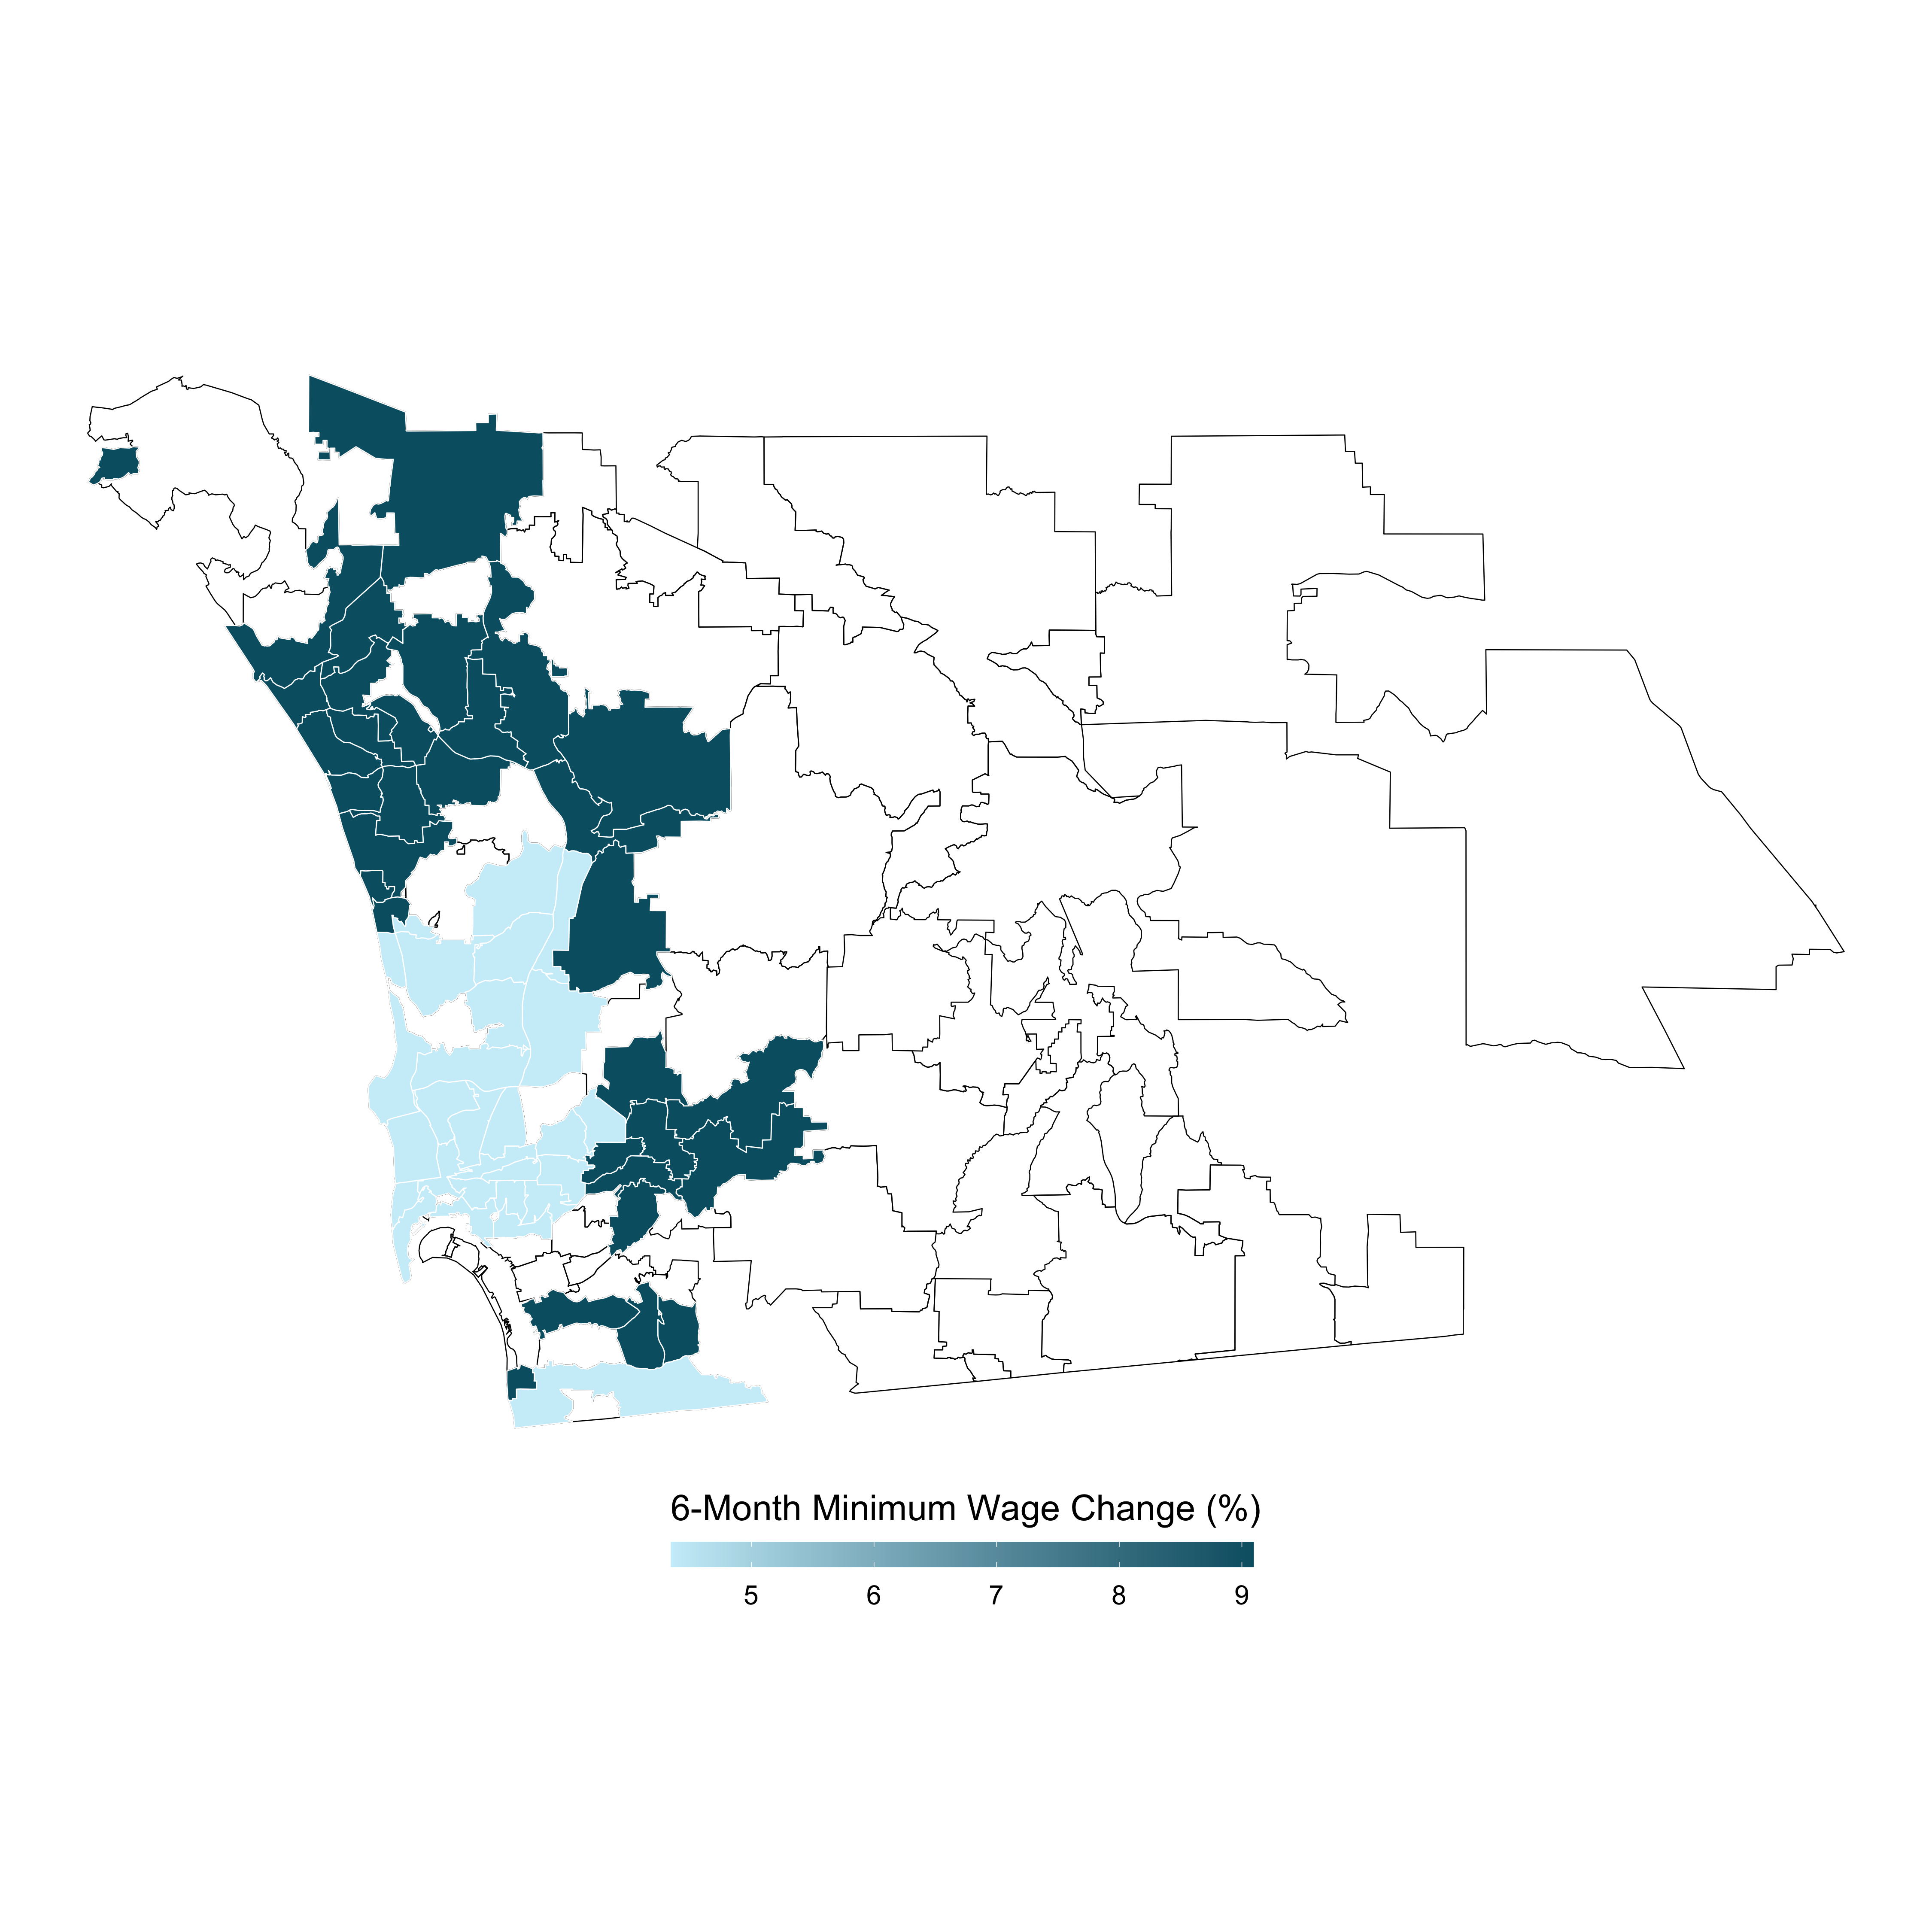
\includegraphics[width = \textwidth]
		{../../analysis/descriptive_maps/output/San_Diego_mw_msa.png}
	\end{subfigure}\\
	\begin{subfigure}[b]{0.65\textwidth}
		\caption{Experienced MW change}
		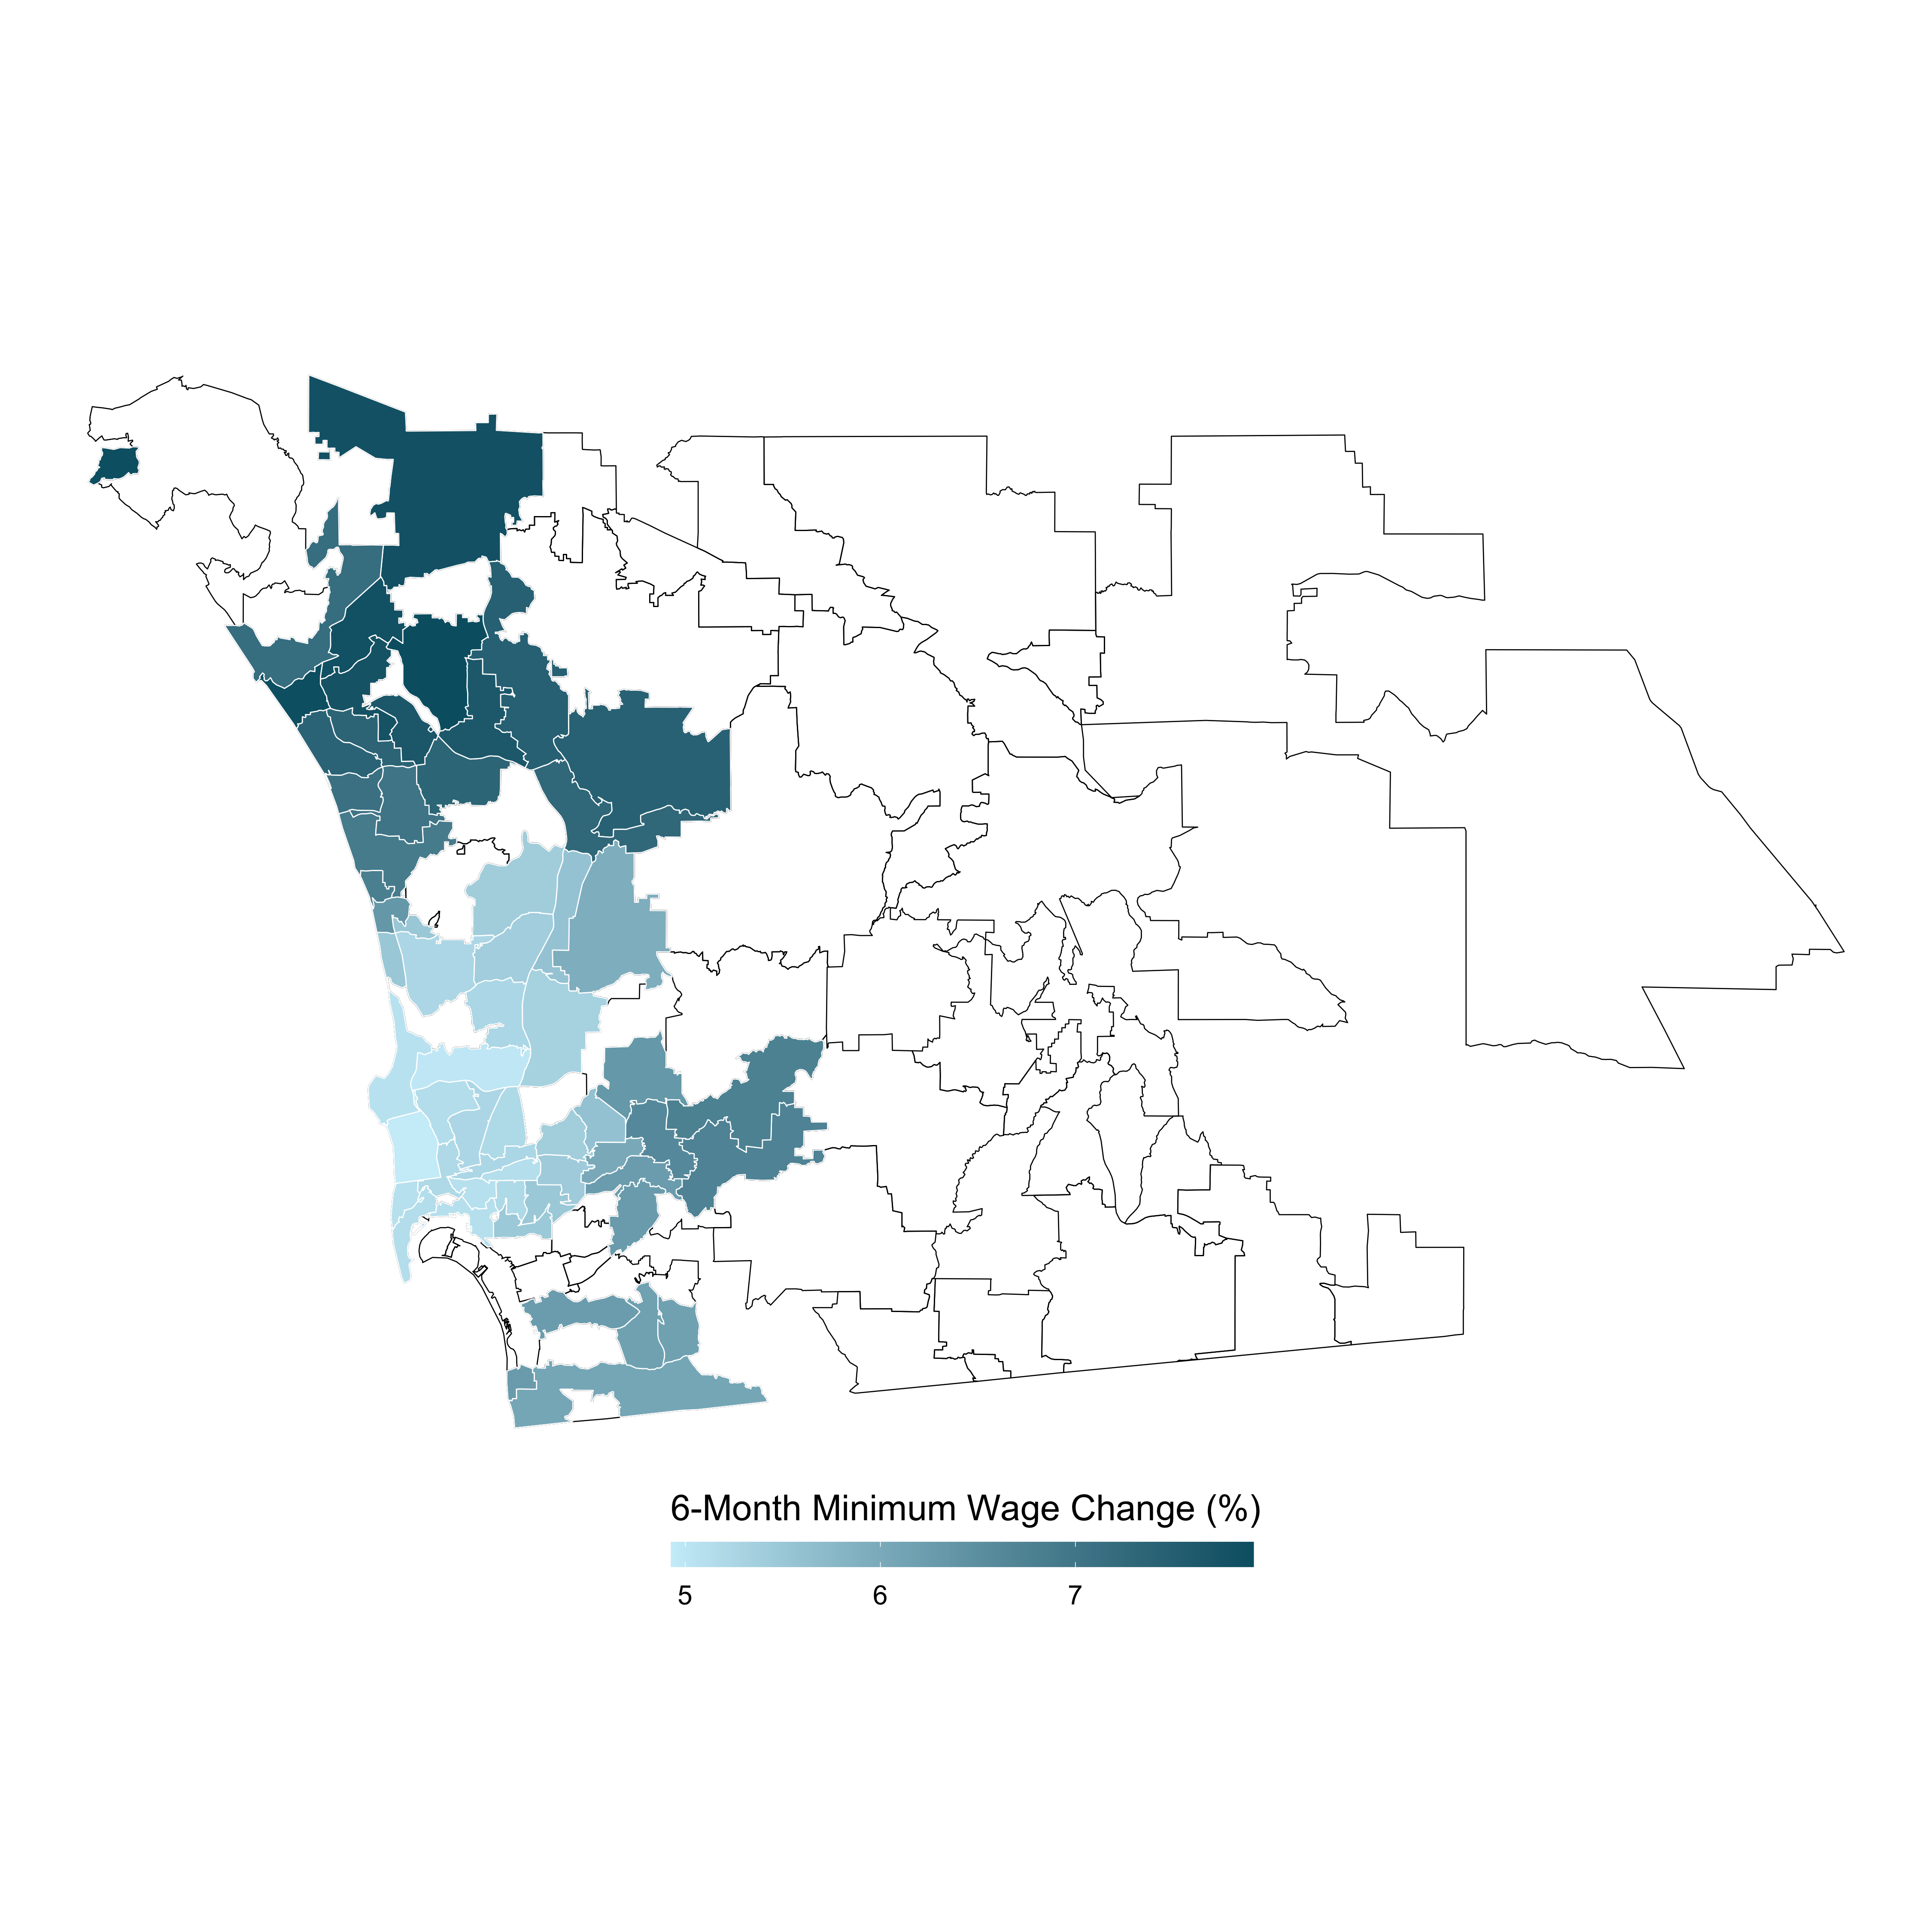
\includegraphics[width = \textwidth]
		{../../analysis/descriptive_maps/output/San_Diego_expmw_msa.png}
	\end{subfigure}
	\begin{minipage}{0.95\textwidth} \footnotesize
		\vspace{2mm} 
		\textit{Notes}: The figure maps the percent increase in our minimum wage and 
		experienced minimum wage measures following the state increase in California
		on January 2019. The map colors only those zipcodes for which we have 
		non-missing rents data from Zillow.
	\end{minipage}
\end{figure}


%%%%%%%%%%%%%%%%%%%%%%%%%%%%%%%%%%%%%%%%%%%%%%%%%%%%%%%%%%%%%%%%%%%%%%%%%%%%%%%%%
\subsection{Estimation results}

We re-estimate our baseline models using the experienced MW as treatment variable and present 
the results in \autoref{tab:expmw_main}. Column 2 shows that both the static and cumulative 
effect on rents slightly increase: a 10 percent increase in the experienced MW leads to a simultaneous
$0.31$ percent rent increase, rising to $0.66$ within 6-months. The higher estimates suggest how 
indeed measurement error is likely to introduce downward bias in baseline results.
%FINISH COMMENT ON RESULTS

%We re-estimate The estimated effect of MW on rents slightly increases in the two statistically significant periods,  
%$t=0$ and $t=1$, but the new results largely confirm the magnitude and dynamics uncovered by the baseline model. 
%A 10 percent increase in experienced MW leads to a $0.31$ percent contemporaneous increase in median rents, as well 
%as a $0.145$ increase in the following month. The absence of statistically significant pre-trend is confirmed.    


\begin{table}[h!]\centering
	\caption{The impact of Experienced Minimum Wage on Rents}
	\label{tab:expmw_main}
	{
\def\sym#1{\ifmmode^{#1}\else\(^{#1}\)\fi}
\begin{tabular}{l*{4}{c}}
\hline\hline
          &\multicolumn{1}{c}{$\Delta \underline{w}_{ict}^{\text{exp}}$}&\multicolumn{3}{c}{$\Delta \ln r_{ict}$}                \\\cmidrule(lr){2-2}\cmidrule(lr){3-5}
          &\multicolumn{1}{c}{(1)}         &\multicolumn{1}{c}{(2)}         &\multicolumn{1}{c}{(3)}         &\multicolumn{1}{c}{(4)}         \\
\hline
$\Delta \ln \underline{w}_{ict}$&   0.8718\sym{***}&   0.0257\sym{*}  &                  &  -0.0320\sym{*}  \\
          & (0.0296)         & (0.0137)         &                  & (0.0163)         \\
[1em]
$\Delta \underline{w}_{ict}^{\text{exp}}$&                  &                  &   0.0320\sym{**} &   0.0662\sym{**} \\
          &                  &                  & (0.0151)         & (0.0278)         \\
\hline
$\Delta \ln \underline{w}_{ict}$ + $\Delta \underline{w}_{ict}^{\text{exp}}$&                  &                  &                  &                  \\
          &                  &                  &                  &                  \\
\vspace{-2mm}&                  &                  &                  &                  \\
Wage controls&      Yes         &      Yes         &      Yes         &      Yes         \\
Employment controls&      Yes         &      Yes         &      Yes         &      Yes         \\
Establishment-count controls&      Yes         &      Yes         &      Yes         &      Yes         \\
P-value equality&                  &                  &                  &    0.027         \\
R-squared &    0.947         &    0.021         &    0.021         &    0.021         \\
Observations&  131,196         &  131,196         &  131,196         &  131,196         \\
\hline\hline
\end{tabular}
}

	\begin{minipage}{\textwidth}\footnotesize
		\vspace{3mm}	
		\textit{Notes:} The table shows the static and cumulative effects caused by a $1$ percent
		change in MW on rents. The static effect is estimated by $\hat{\beta}$ from \autoref{eq:did};
		the cumulative effect is obtained as a linear combination of the $\beta_{t+r}$ coefficients from 
		a distributed-lags model based on \autoref{eq:leads_lags}: 
		$\sum\limits_{r = 0}^5 \hat{\beta}_{t+r}$. All specifications include time fixed effects, 
		and additionally use QCEW data to control for wages, employment and number of establishments 
		for the ``Professional and business services", ``Information", and ``Financial activities" industries.
		Standard errors clustered at the state level are
		reported in parenthesis. \\
		Significance codes: *** $p < 0.01$, ** $p < 0.05$, * $p < 0.1$. 	
	\end{minipage}
\end{table}



